% Cole Nielsen niels538@umn.edu
% EE 2002 Spring 2015
% Formal Lab Report 1

%----------------------------------------------------------------------------------------
%	PACKAGES AND DOCUMENT CONFIGURATIONS
%----------------------------------------------------------------------------------------

\documentclass[12pt]{article}

\usepackage{circuitikz}
\usepackage{graphicx}
\usepackage{subcaption}
\usepackage[top=1in, bottom= 1in, left=1in, right= 1in]{geometry}
\setlength\parindent{0pt}
\usepackage{fancyhdr}
\pagestyle{fancy}
\usepackage{textcomp}
\usepackage{tikz}
%\usepackage{cmbright}
%\usepackage[T1]{fontenc}
\usepackage{siunitx}
\usepackage{placeins}
\usepackage{titlesec}
\usepackage{cancel} 
\usepackage{adforn}
\ctikzset{tripoles/mos style/arrows}
\tikzset{srail/.style={sground,yscale=-1}}
\fancyfoot{} % clear all footer fields
\renewcommand{\footrulewidth}{0.4pt}
\fancyfoot[LE,CO]{\thepage}
\fancyfoot[LE,LO]{High Speed Camera Proposal} %DOCUMENT NUMBER
\fancyfoot[LE,RO]{\today} %REVISION DATE - FORMAT: CN####-X
\setlength{\parskip}{0.75em} 
%----------------------------------------------------------------------------------------
%	DOCUMENT INFORMATION
%----------------------------------------------------------------------------------------

\title{\LARGE Low-Cost High-Speed Video Camera\\\adforn{21}\\Envision Fund Proposal}


\date{}

\begin{document}
\maketitle 
\begin{center}
 \begin{tabular}{l r}
   Cole \textsc{Nielsen} & niels538@umn.edu\\ 
   Mason \textsc{Tran}: & tranx801@umn.edu\\ 
\end{tabular}
\end{center}
\pagebreak
%----------------------------------------------------------------------------------------
%	Abstract
%----------------------------------------------------------------------------------------
%\begin{abstract}
%\noindent 

%\end{abstract}
%\hrulefill
%----------------------------------------------------------------------------------------
%	Introduction
%----------------------------------------------------------------------------------------
\section{Introduction}
High speed video cameras have typically been high cost devices, due to requirements for speed data storage systems and imaging sensors required to build them. This has essentially prohibited access to high-video equipment to those outside of research environments. In the last decade, however, cost for high speed data storage has dropped significantly due to introduction of relatively cheap and high speed DDR3 RAM. The availability of cheap FPGAs supporting DDR3 RAM has further spurred the possibility of implementing a data storage system capable of the speeds needed for affordable high speed video. Despite this, the cost of high speed imaging sensors have remained prohibitively expensive until recently. In 2015, ON Semiconductor introduced the PYTHON series of high speed imaging sensors, with the low end VGA (640x480) resolution PYTHON300 costing under \$60, yet is capable of delivering 2235 FPS (frames per second) of video aquisiton at 256x256 resolution. At lower resolutions the PYTHON300 is capable of even higher frame rates, for example at 64x64 resolution 16,500 FPS is achievable. Viewed at 30 FPS, the 16,500 FPS video is effectively slowed down by 550x. Finally, with the availability of these low cost sensors, the possibily of constructing high speed video camera has become possible. \\\par

Therefore, we are making this proposal to the Envision Fund in order to design and construct a high speed video camera utilizing PYTHON300 sensor, with a DDR3 RAM and Cyclone V FPGA based memory system. We are also proposing to integrate a Raspberry Pi Zero with LCD into the camera as the user interface, allowing video playback to be directly viewed on the camera. We believe this project is an excellent cantidate for Envision Fund funding, as it is a challanging design, as well as an innovative one, bringing high speed video at low costs. From a DIY standpoint this project is attractive as few DIY high speed cameras have been built, so it stands as a way to open the electronics community to this technology. The further sections of this proposal lay out a more detailed plan for the technical design, cost (approx. \$360) and timeline for the project.

\section{Technical Details}
The basis of this design in the PYTHON300 sensor. We plan to use the NOIP1SN0300A-QDI variant, which a VGA resolution monochrome sensor. Monochrome was chosen over color as monochrome sensors inherently have higher effective resolution and sensitivity than color sensors. This means the camera will be able to work in far lower light and distinguish finer details than if a equivalent color sensor were be used. The sensor will be controlled by a Cyclone V FPGA, with a NIOS-II soft processor sending SPI commands to control the sensor. The sensor will output a maximum of 288 Megapixels/second over four LVDS data lines to the FPGA. With each pixel outputted at 1 byte of data, the throughput to the FPGA per data line will be at most 576 Mbps, which is well within the 700 Mbps capability of the FPGA. The FPGA will then store the image data real time to the DDR3 RAM. The DDR3 RAM is planned to be comprised of two 4Gb chips, each capable of storing 512 megabytes, or equivalenly 512 megapixels of data. From the data in the PYTHON300 datasheet, the follow record times at the given resolutions below will be possible with this memory:

\begin{table}[h]
 \renewcommand\tabcolsep{12pt}
\renewcommand{\arraystretch}{1.25}
\centering
\begin{tabular}{lll}
\hline\hline
\textbf{Resolution} & \textbf{Frame Rate (FPS)} & \textbf{Record time}\\ 
\hline 
640x480 (VGA) & 815 FPS & 4.3 seconds\\ 
\hline 
256 x 256 & 2235 FPS & 7.3 seconds\\ 
\hline 
64x64 & 16,500 FPS & 15.9 seconds\\ 
\hline 
\end{tabular}
\label{table:name}
\end{table}
Maximum data rate decreases with frame rate, so we see that record time increases with frame rate. Once a video is done recording, it is to be transferred via USB to the Raspberry Pi Zero, which is a small single board Linux computer, where the video will be encoded into a standard video format and then stored onto the Raspberry Pi's onboard SD card. A resistive touch LCD display interfaced to the Raspberry Pi will be used to interact with and control the camera. A simple application will be displayed on the screen, allowing configuring the settings of the camera, initiating recording and playback of recorded videos. Below is a block diagram showing the basic design described of the high speed camera:
\begin{center}
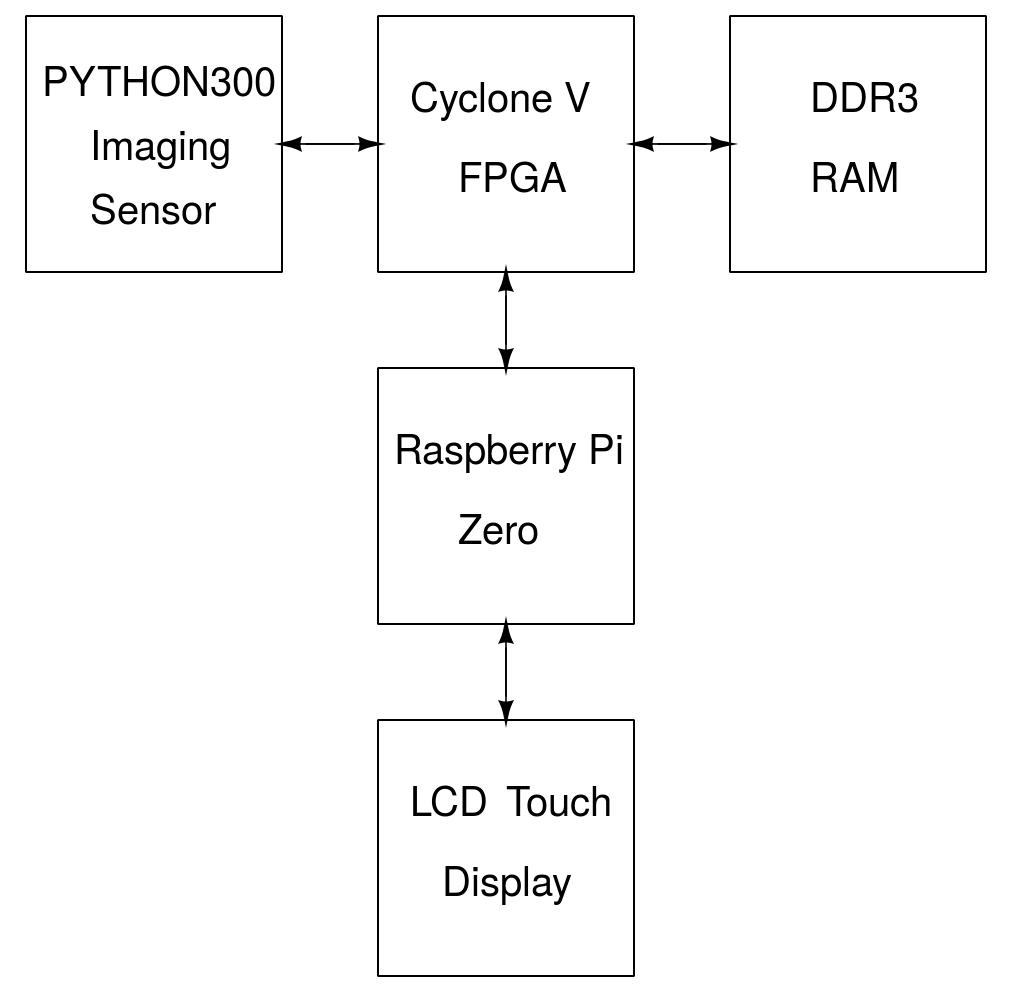
\includegraphics[width=3in]{hsc.png}
\end{center}
The camera is planned to be built as a single four-layer PCB integrating the image sensor, FPGA, RAM and supporting electronics on one board. It will be designed in Altium Designer and manufactured by Osh Park. The device will be housed in a 3d printed box having a C-mount camera lens fixed to the front, which will project an image inside the box onto the imaging sensor. The Rasberry Pi zero and LCD will be mounted inside the box, on the face opposite of the lens. The final product aproximately be a 3x3x3 inch cube (not including lens). 
\section{Cost}
Below is a table giving a preliminary cost estimate of the project:
\begin{table}[h]
 \renewcommand\tabcolsep{12pt}
\renewcommand{\arraystretch}{1.25}
\centering
\begin{tabular}{lll}
\hline\hline
\textbf{Item} & \textbf{Cost}\\ 
\hline 
PYTHON300 Sensor (NOIP1SN0300A-QDI)& \$55.50\\ 
\hline 
DDR3 RAM (2x AS4C512M8D3L-12BIN) & \$23.30 \\ 
\hline 
Cyclone V FPGA (5CEBA2F17C8N) & \$34.81 \\ 
\hline 
Additional PCB components & \$25 \\ 
\hline 
5 in$^2$ four layer PCB & \$50.00 \\ 
\hline 
Raspberry Pi and LCD & \$50.00 \\ 
\hline 
3d Printed Box & \$50.00\\
\hline
25 mm C-Mount Lens& \$25 \\ 
\hline 
Other costs & \$50.00 \\ 
\hline\hline 
\textbf{TOTAL}& \textbf{\$363.81} \\ 
\hline 
\end{tabular}
\end{table}
\section{Project Timeline}
Below is the project timeline given in phases (assumed after funding approved):\\\par 
\subsection*{\normalsize Phase 1: 3 weeks}
Design circuit/schematic, layout PCB, design mechanical assembly in CAD. At end of phase submit PCB to be manufactured and box to be 3d printed. Components will also be ordered at end of phase.
\subsection*{\normalsize Phase 2a: 1 weeks}
Code preliminary hardware description in Verilog for the data controller, write image sensor control program for NIOS II soft core.
\subsection*{\normalsize Phase 2b: 4 weeks}
Once parts, PCB and box received, assemble the camera and then begin the primary phase of the FPGA development. Outcome will be a functioning system that is able to control the imaging sensor, store image data to RAM and then transmit the stored data over USB to a computer.
\subsection*{\normalsize Phase 3: 4 weeks}
Develop application for Raspberry Pi that (a) can communicate with the camera board over USB, (b) convert the raw video data to a standard video format, (c) display a live video view, (d) replay recorded video and (e) control the camera settings and start video recording.
\end{document}